\chapter{Computational Algebra and Similarity}
\label{ch:algebra}

\section{Buchberger's Algorithm}
\label{sec:buchbergers_algorithm}

\subsection{Overview}
Buchberger's algorithm is a fundamental method in computational algebraic geometry for computing a \textbf{Gr\"obner basis} of a polynomial ideal\index{Gr\"obner basis}\index{Buchberger's algorithm}. Much like the Gaussian elimination algorithm for linear systems, Buchberger's algorithm transforms a set of multivariate polynomials into a ``standard'' form that makes it easy to solve systems of equations, perform polynomial division, and analyze the properties of the underlying algebraic variety. The algorithm was first described by Bruno Buchberger in his 1965 PhD thesis~\cite{buchberger1965} and has since become a cornerstone of computational algebra, extensively treated in standard references such as Cox, Little, and O'Shea~\cite{cox2007}.

\subsection{Definitions}

\begin{definition}[Polynomial Ideal]\label{def:polynomial_ideal}
Let $k$ be a field and let $f_1, \dots, f_m \in k[x_1, \dots, x_n]$ be a set of polynomials. The \textbf{polynomial ideal}\index{polynomial ideal} generated by these polynomials is the set
\[
I = \langle f_1, \dots, f_m \rangle = \left\{ \sum_{i=1}^{m} h_i f_i \;\middle|\; h_i \in k[x_1, \dots, x_n] \right\}.
\]
The polynomials $f_1, \dots, f_m$ are called the \emph{generators} of~$I$.
\end{definition}

\begin{definition}[Monomial Order]\label{def:monomial_order}
A \textbf{monomial order}\index{monomial order} on $k[x_1, \dots, x_n]$ is a total ordering $\succ$ on the set of monomials $x^{\alpha} = x_1^{\alpha_1} \cdots x_n^{\alpha_n}$ (where $\alpha \in \mathbb{N}^n$) that satisfies:
\begin{enumerate}
    \item $x^{\alpha} \succ 1$ for all $\alpha \neq \mathbf{0}$.
    \item If $x^{\alpha} \succ x^{\beta}$, then $x^{\alpha + \gamma} \succ x^{\beta + \gamma}$ for all $\gamma \in \mathbb{N}^n$.
\end{enumerate}
Common choices include \textbf{lexicographic} (Lex) and \textbf{graded reverse lexicographic} (Degrevlex). For two monomials $x^{\alpha}$ and $x^{\beta}$, the Lex order compares first by $x_1$-exponent, then $x_2$, etc., while Degrevlex first compares by total degree and then breaks ties by the last differing exponent in reverse.
\end{definition}

\begin{definition}[Leading Term]\label{def:leading_term}
Given a monomial order $\succ$ and a nonzero polynomial $f = \sum_{\alpha} c_{\alpha} x^{\alpha}$, the \textbf{leading term} $\operatorname{LT}(f)$ is the term $c_{\alpha} x^{\alpha}$ with the greatest $\alpha$ under~$\succ$. Similarly, $\operatorname{LM}(f)$ denotes the leading monomial (coefficient removed) and $\operatorname{LC}(f)$ the leading coefficient.
\end{definition}

\begin{definition}[Gr\"obner Basis]\label{def:grobner_basis}
A finite set $G = \{g_1, \dots, g_t\} \subset I$ is a \textbf{Gr\"obner basis}\index{Gr\"obner basis} for the ideal $I = \langle f_1, \dots, f_m \rangle$ with respect to a monomial order $\succ$ if
\[
\langle \operatorname{LT}(g_1), \dots, \operatorname{LT}(g_t) \rangle = \langle \operatorname{LT}(I) \rangle,
\]
where $\operatorname{LT}(I) = \{\operatorname{LT}(f) \mid f \in I \setminus \{0\}\}$ is the set of all leading terms of nonzero polynomials in~$I$.
\end{definition}

\begin{definition}[S-Polynomial]\label{def:s_polynomial}
Given two nonzero polynomials $f, g$ and a monomial order $\succ$, the \textbf{S-polynomial}\index{S-polynomial} is defined as
\[
S(f, g) = \frac{L}{\operatorname{LT}(f)} f - \frac{L}{\operatorname{LT}(g)} g,
\]
where $L = \operatorname{lcm}(\operatorname{LM}(f), \operatorname{LM}(g))$ is the least common multiple of the leading monomials of $f$ and $g$. The S-polynomial is constructed precisely to cancel the leading terms of $f$ and $g$.
\end{definition}

\subsection{Theory}
\label{subsec:buchberger_theory}

The algorithm starts with an initial set of generators $G$. It systematically checks all pairs of polynomials $(f, g)$ in $G$ and calculates their S-polynomial:
$$S(f, g) = \frac{L}{LT(f)} f - \frac{L}{LT(g)} g$$
where $L = \text{lcm}(LM(f), LM(g))$.

The S-polynomial is then reduced by the current basis $G$ using multivariate polynomial division. If the remainder is non-zero, it means $G$ is not yet a Gr\"obner basis, and the remainder is added to $G$. This process continues until the S-polynomial of every pair in $G$ reduces to zero.

\begin{theorem}[Buchberger's Criterion]\label{thm:buchberger_criterion}
A finite generating set $G$ for an ideal $I$ is a Gr\"obner basis with respect to a monomial order $\succ$ if and only if for every pair $f_i, f_j \in G$, the remainder of the S-polynomial $S(f_i, f_j)$ on division by $G$ is zero; that is, $S(f_i, f_j) \xrightarrow{G} 0$ for all $i \neq j$.
\end{theorem}

\begin{proof}
The forward direction is straightforward: if $G$ is a Gr\"obner basis, then $\operatorname{LT}(G)$ generates $\operatorname{LT}(I)$, so every $S$-polynomial reduces to zero by the division algorithm. The converse relies on the fact that if $S(f_i, f_j) \to 0$ for all pairs, then the leading terms of $G$ generate $\operatorname{LT}(I)$, which is shown by induction on the monomial order applied to an arbitrary $h \in I$; see~\cite[Chapter~2]{cox2007} for the complete proof.
\end{proof}

\begin{theorem}[Termination of Buchberger's Algorithm]\label{thm:buchberger_termination}
Buchberger's algorithm terminates after finitely many steps for any input set of polynomials $F$ and any admissible monomial order.
\end{theorem}

\begin{proof}
Each time a nonzero remainder $r$ is produced, $r$ is added to $G$, and $\langle \operatorname{LT}(G) \rangle$ strictly increases in the monomial ideal lattice. Since every monomial ideal is finitely generated (by Dickson's lemma), this chain of strict inclusions must stabilize, and the algorithm terminates.
\end{proof}

\begin{figure}[htbp]
\centering
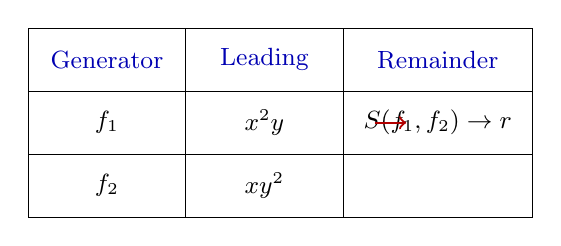
\begin{tikzpicture}[scale=0.8]
  \draw (0,0) rectangle (8,3);
  \draw (0,1)--(8,1);
  \draw (0,2)--(8,2);
  \draw (2.5,0)--(2.5,3);
  \draw (5,0)--(5,3);
  \node[font=\small,blue!70!black] at (1.25,2.5) {Generator};
  \node[font=\small,blue!70!black] at (3.75,2.5) {Leading};
  \node[font=\small,blue!70!black] at (6.5,2.5) {Remainder};
  \node[font=\small] at (1.25,1.5) {$f_1$};
  \node[font=\small] at (1.25,0.5) {$f_2$};
  \node[font=\small] at (3.75,1.5) {$x^2 y$};
  \node[font=\small] at (3.75,0.5) {$xy^2$};
  \node[font=\small] at (6.5,1.5) {$S(f_1,f_2) \to r$};
  \draw[->,thick,red!70!black] (5.5,1.5)--(6,1.5);
\end{tikzpicture}
\caption{Buchberger's algorithm: S-polynomials are formed from pairs of generators and reduced.}
\label{fig:grobner}
\end{figure}


\subsection{Pseudocode}
\begin{algorithm}[ht]
\label{alg:buchberger}
\begin{algorithmic}[1]
\Function{Buchberger}{$F$, monomial\_order}
    \State $G \gets F$
    \State $\text{pairs} \gets \{(f_i, f_j) \mid f_i, f_j \in G,\; i < j\}$
    \While{$\text{pairs} \neq \emptyset$}
        \State $(f, g) \gets \text{pairs.pop}()$
        \State $S \gets \text{S\_Polynomial}(f, g, \text{monomial\_order})$
        \State $\text{remainder} \gets \text{MultivariateDivision}(S, G, \text{monomial\_order})$
        \If{$\text{remainder} \neq 0$}
            \For{each $\text{existing\_g}$ in $G$}
                \State $\text{pairs.add}((\text{existing\_g}, \text{remainder}))$
            \EndFor
            \State $G.\text{append}(\text{remainder})$
        \EndIf
    \EndWhile
    \State \Return $G$
\EndFunction
\end{algorithmic}
\end{algorithm}

\begin{example}[Computing an S-Polynomial]\label{ex:s_polynomial}
Let $f = x^2 y - 1$ and $g = xy^2 - 1$ with Lex order ($x \succ y$). Then $\operatorname{LT}(f) = x^2 y$ and $\operatorname{LT}(g) = xy^2$, so $L = \operatorname{lcm}(x^2 y, xy^2) = x^2 y^2$. The S-polynomial is
\[
S(f, g) = \frac{x^2 y^2}{x^2 y} f - \frac{x^2 y^2}{xy^2} g = y \cdot f - x \cdot g = (x^2 y^2 - y) - (x^2 y^2 - x) = x - y.
\]
Since $x - y$ is nonzero, it would be added to the basis $G$ during \cref{alg:buchberger}.
\end{example}

\subsection{Parameter Selection}
\begin{itemize}
    \item \textbf{Monomial Order}: \textbf{Lexicographic} (Lex) is used for solving systems of equations, while \textbf{Graded Reverse Lexicographical} (Degrevlex)\index{Degrevlex} is generally much faster for computing the basis.
    \item \textbf{Selection Heuristic}: Choosing pairs with the smallest LCM of leading terms can improve performance.
\end{itemize}

\subsection{Complexity}
\begin{itemize}
    \item \textbf{Time Complexity}: In the worst case, the algorithm's complexity can be \textbf{doubly exponential} in the number of variables~$n$. More precisely, for a zero-dimensional ideal with $n$ variables and maximum degree $d$, the number of polynomials in a Gr\"obner basis can be $O(d^{2^n})$.
    \item \textbf{Space Complexity}: Can also grow extremely large as many intermediate polynomials are generated.
\end{itemize}

\subsection{Usages}
\begin{itemize}
    \item \textbf{Solving Polynomial Systems}: Transforming a complex system into a Lex-ordered Gr\"obner basis (which looks like a ``triangular'' system) and solving by back-substitution.
    \item \textbf{Surface Implicitization}\index{surface implicitization}: Converting a parametric surface (e.g., B\'ezier or NURBS) into an implicit equation $f(x, y, z) = 0$.
    \item \textbf{Collision Detection}: Determining if two curved surfaces (defined by algebraic equations) intersect.
    \item \textbf{Robot Kinematics}: Solving the inverse kinematics problem for robot arms with multiple joints.
    \item \textbf{Motion Planning}: Checking for intersections between objects in configuration space.
\end{itemize}

\subsection{Testing Methods and Edge Cases}
\begin{itemize}
    \item \textbf{Linear Systems}: On a system of linear equations, Buchberger should perform identically to Gaussian elimination.
    \item \textbf{Single Variable}: On polynomials in $x$, it should behave like the Euclidean algorithm for finding the GCD.
    \item \textbf{Inconsistent Systems}: If the system has no solution, the Gr\"obner basis should contain the constant~1.
    \item \textbf{Redundant Generators}: The algorithm should eliminate redundant polynomials.
    \item \textbf{Monomial Order Sensitivity}: Verify that the resulting basis is correct for different orders (Lex vs.\ Degrevlex).
\end{itemize}

\subsection{References}
\begin{itemize}
    \item Buchberger, B. (1965). ``An Algorithm for Finding the Basis Elements of the Residue Class Ring of a Zero Dimensional Polynomial Ideal''. PhD Thesis.
    \item Cox, D., Little, J., \& O'Shea, D. (2007). ``Ideals, Varieties, and Algorithms''. Springer.
    \item Wikipedia: \href{https://en.wikipedia.org/wiki/Buchberger\%27s_algorithm}{Buchberger's algorithm}
\end{itemize}

\section{Resultant-Based Elimination}
\label{sec:resultant_elimination}

\subsection{Overview}
Resultant-based elimination is a symbolic algebraic technique used to eliminate variables from a system of polynomial equations\index{resultant}\index{Sylvester matrix}. The \textbf{resultant} of two polynomials is a scalar value (or another polynomial) that is zero if and only if the two original polynomials share a common root. This concept dates to the work of Sylvester~\cite{sylvester1840} and has been extensively developed in modern computational algebra~\cite{cox2007}. By calculating the resultant with respect to one variable, we ``project'' the intersection of the two polynomials onto a lower-dimensional space. It is a faster alternative to Gr\"obner bases for many problems in surface implicitization and collision detection~\cite{manocha1994}.

\subsection{Definitions}

\begin{definition}[Resultant]\label{def:resultant}
Let $f(x) = a_n x^n + \cdots + a_0$ and $g(x) = b_m x^m + \cdots + b_0$ be two polynomials in $k[x]$ with coefficients in a field $k$. The \textbf{resultant}\index{resultant} $\operatorname{Res}(f, g, x)$ is a polynomial in the coefficients $a_i, b_j$ that vanishes if and only if $f$ and $g$ have a common root in some extension field of $k$, or equivalently, $\gcd(f, g)$ has positive degree.
\end{definition}

\begin{definition}[Sylvester Matrix]\label{def:sylvester_matrix}
For $f(x) = a_n x^n + \cdots + a_0$ and $g(x) = b_m x^m + \cdots + b_0$, the \textbf{Sylvester matrix}\index{Sylvester matrix} is the $(m+n) \times (m+n)$ matrix formed by stacking $m$ shifted copies of the coefficient vector of $f$ followed by $n$ shifted copies of the coefficient vector of $g$:
\[
\mathbf{S}(f,g) = \begin{pmatrix}
a_n & a_{n-1} & \cdots & a_0 & 0 & \cdots & 0 \\
0 & a_n & a_{n-1} & \cdots & a_0 & \cdots & 0 \\
\vdots & & \ddots & & & \ddots & \vdots \\
0 & \cdots & 0 & a_n & a_{n-1} & \cdots & a_0 \\
b_m & b_{m-1} & \cdots & b_0 & 0 & \cdots & 0 \\
0 & b_m & b_{m-1} & \cdots & b_0 & \cdots & 0 \\
\vdots & & \ddots & & & \ddots & \vdots \\
0 & \cdots & 0 & b_m & b_{m-1} & \cdots & b_0
\end{pmatrix}
\]
The resultant is $\operatorname{Res}(f,g,x) = \det(\mathbf{S}(f,g))$.
\end{definition}

\begin{definition}[Elimination]\label{def:elimination}
\textbf{Elimination}\index{elimination} is the process of reducing a system of $n$ polynomial equations in $n$ variables to a system of fewer variables. In the context of resultants, computing $\operatorname{Res}_x(f, g)$ eliminates the variable $x$, yielding a polynomial in the remaining variables whose roots encode the $x$-coordinates of intersection points.
\end{definition}

\subsection{Theory}

The resultant of two polynomials $f(x) = \sum a_i x^i$ and $g(x) = \sum b_j x^j$ is the determinant of the Sylvester matrix.

For example, if $f(x, y)$ and $g(x, y)$ are two implicit curves, their resultant $\text{Res}_x(f, g)$ is a polynomial in $y$ whose roots are the $y$-coordinates of all intersection points. This allows us to solve for $y$ first and then back-substitute to find $x$.

For \textbf{Implicitization}\index{implicitization}, given parametric equations $x = X(t)$, $y = Y(t)$, $z = Z(t)$, we form the polynomials $f_1 = x - X(t)$, $f_2 = y - Y(t)$, $f_3 = z - Z(t)$ and calculate the resultant $\text{Res}_t(f_1, f_2, f_3)$ to eliminate the parameter~$t$.

\begin{theorem}[Resultant Characterization]\label{thm:resultant}
Let $f, g \in k[x]$ be nonzero polynomials of degrees $n$ and $m$ respectively. Then $\operatorname{Res}(f, g, x) = 0$ if and only if $f$ and $g$ have a common root in the algebraic closure $\overline{k}$, or both $\operatorname{LC}(f) = 0$ and $\operatorname{LC}(g) = 0$.
\end{theorem}

\begin{proof}
The result follows from the equivalence: $f$ and $g$ share a common root if and only if there exist nonzero polynomials $u, v$ with $\deg(u) < m$ and $\deg(v) < n$ such that $u f + v g = 0$. This linear system in the coefficients of $u$ and $v$ has a nontrivial solution if and only if the $(m+n) \times (m+n)$ Sylvester matrix is singular, which occurs precisely when its determinant (the resultant) is zero. See~\cite[Chapter~3]{cox2007}.
\end{proof}

\begin{example}[Resultant of Two Quadratics]\label{ex:resultant_quadratic}
Let $f(x) = x^2 + px + q$ and $g(x) = x^2 + rx + s$ (both degree $n = m = 2$). The Sylvester matrix is $4 \times 4$:
\[
\mathbf{S} = \begin{pmatrix}
1 & p & q & 0 \\
0 & 1 & p & q \\
1 & r & s & 0 \\
0 & 1 & r & s
\end{pmatrix}
\]
Computing the determinant:
\[
\operatorname{Res}(f, g, x) = (q - s)^2 - (p - r)(ps - qr).
\]
Setting this to zero yields the condition under which the two quadratics share a root.
\end{example}

\subsection{Pseudocode}
\begin{algorithm}[ht]
\label{alg:resultant}
\begin{algorithmic}[1]
\Function{Resultant}{$f$, $g$, $x$}
    \State $S \gets \text{BuildSylvesterMatrix}(f, g, x)$
    \State $\text{res} \gets \text{determinant}(S)$
    \State \Return $\text{res}$
\EndFunction

\Function{BuildSylvesterMatrix}{$f$, $g$, $x$}
    \State Build matrix rows by shifting the coefficient vectors:
    \State $[a_n, a_{n-1}, \ldots, a_0, 0, 0]$
    \State $[0, a_n, a_{n-1}, \ldots, a_0, 0]$
    \State $\vdots$
    \State $[b_m, b_{m-1}, \ldots, b_0, 0, 0]$
    \State $[0, b_m, b_{m-1}, \ldots, b_0, 0]$
    \State \Return $S$
\EndFunction
\end{algorithmic}
\end{algorithm}

\subsection{Parameter Selection}
\begin{itemize}
    \item \textbf{Matrix Type}: Sylvester matrices are large and sparse. Bezout or Dixon matrices are much smaller for higher-order polynomials but are more complex to construct.
    \item \textbf{Numerical Precision}: If coefficients are floating-point numbers, calculating the determinant can be numerically unstable. Using symbolic computation or arbitrary-precision arithmetic is recommended.
\end{itemize}

\subsection{Complexity}
\begin{itemize}
    \item \textbf{Time Complexity}: $O(d^3)$ where $d = \deg(f) + \deg(g)$, based on the cost of the determinant calculation of the $(m+n) \times (m+n)$ Sylvester matrix.
    \item \textbf{Space Complexity}: $O(d^2)$ to store the Sylvester matrix.
\end{itemize}

\subsection{Usages}
\begin{itemize}
    \item \textbf{Surface Implicitization}: Converting parametric B\'ezier/NURBS surfaces into implicit $f(x, y, z) = 0$ equations for faster inside/outside tests.
    \item \textbf{Curve/Surface Intersection}: Finding the exact points where a line (ray) intersects a curved surface.
    \item \textbf{Collision Detection}: Determining if two curved objects intersect by checking if their resultant has any real roots.
    \item \textbf{Robot Kinematics}: Solving inverse kinematics for complex linkages.
    \item \textbf{Computer Aided Design (CAD)}: Boolean operations on curved surfaces.
\end{itemize}

\subsection{Testing Methods and Edge Cases}
\begin{itemize}
    \item \textbf{Two Lines}: The resultant of two linear equations $a_1 x + b_1$ and $a_2 x + b_2$ should be $a_1 b_2 - a_2 b_1$.
    \item \textbf{Parallel Curves}: If curves never intersect, the resultant should be a non-zero constant.
    \item \textbf{Coincident Curves}: If two curves are the same, the resultant will be identically zero.
    \item \textbf{Leading Coefficient Zero}: Ensure the algorithm handles cases where the leading coefficient vanishes for certain values of the other variables.
    \item \textbf{Large Degrees}: Verify that the determinant calculation remains robust for polynomials of degree 10+.
\end{itemize}

\subsection{References}
\begin{itemize}
    \item Sylvester, J.~J. (1840). ``A method of determining by inspection the form of the combined roots of two algebraic equations''. Philosophical Magazine.
    \item Cox, D., Little, J., \& O'Shea, D. (2007). ``Ideals, Varieties, and Algorithms''. Springer.
    \item Manocha, D. (1994). ``Solving systems of polynomial equations using resultants''. SIGGRAPH Course.
    \item Wikipedia: \href{https://en.wikipedia.org/wiki/Resultant}{Resultant}
\end{itemize}
